\chapter{Theoretical introduction}
\label{chap:intro}

In this chapter, we introduce concepts essential for understanding this thesis' concerns. The first subsection is aimed to deliver the basic characterization of CCs. In the following subsection, we talk about the motion of a charged particle in rapidly changing fields. Next, we will introduce the idea of laser cooling. And finally, in the last subsection, we propose our design of an experiment capable of achieving simultaneous electron-ion trapping and cooling.

\section{Coulomb crystal}
Most of the solid matter we come across has either a crystal or rather polycrystal structure. Meaning its elementary constituents (atoms, molecules, ions) create an ordered formation repeating itself, in the case of crystals up to macroscopic scales. The shape of these structures \cite{drewsen2003ion} is essentially dictated by the atomic wave function overlap. A CC orders itself differently. An average distance between ions in a CC is usually \cite{thompson2015ion} five orders of magnitude larger than it is for atoms in typical matter. On this scale are quantum effects negligible, and ions are merely pushed away from each other by classical Coulomb interaction. Therefore they need an external force to keep them together, which is provided by a trapping potential in our case. However, these structures can also be found in nature, namely in the cores of white dwarfs and crusts of neutron stars.

\subsubsection{Plasma}
Not all texts agree on a precise definition of plasma. A somewhat broad definition \cite{fitzpatrick2014plasma} states that plasma is an ionized gas exerting collective behavior. We often demand quasineutrality as well, suggesting similar ion and electron concentrations. By this merit, a CC can not be labeled plasma as it is composed exclusively of positive ions. Collective behavior means the plasma responds to external macroscopic stimuli as a whole. The standard parameter linked to this aspect is plasma frequency $\omega_p$, describing how quickly plasma reacts to the imposed electromagnetic field.
\begin{equation}
	\label{plasma frequency}
	\omega_p = \frac{n Q^2}{\varepsilon_0 M},
\end{equation}
where $n$ represents a concentration of charged particles, $Q$ their charge, $M$ their mass, and $\varepsilon_0$ is the vacuum permittivity. This equation \eqref{plasma frequency} shows that the electrons play an essential role in collective behavior, as they can react much more swiftly than heavy ions. That is another reason it is necessary to add electrons so that CC can become plasma.

Plasma can have multiple components, each having different masses and velocities. We define a temperature \cite{fitzpatrick2014plasma} for each species individually as their mean kinetic energy:
\begin{equation}
	\label{temperature}
	k_b T_s = \frac{1}{3} M_s \langle v_s^2 \rangle,
\end{equation}
where $\langle v_s \rangle$ denotes an average velocity of single species, and $k_b$ is a Boltzmann constant.

Another crucial attribute when examining plasma is the $\Gamma$ parameter, representing the proportion of Coulomb potential energy to the plasma's kinetic energy.
\begin{equation}
	\label{gamma def}
	\Gamma \equiv \frac{E_c}{k_b T},
\end{equation}
where $T$ denotes temperature, and $E_c$ Coulomb energy. It is not easy to figure out the potential energy of a general plasma. However, when dealing with Coulomb crystals composed of tens to hundreds of ions, nothing stops us from computing it exactly. Classical thermal plasma has $k_b T \gg E_c$. In the case of CCs, $k_b T < E_c$ and we are talking about \emph{strongly coupled} plasma.

\section{Ion trapping}
Here we introduce the concept of trapping a single ion by a quickly oscillating field. We will tightly follow a classic textbook \cite{gerlich1992inhomogeneous} in the whole section, starting by writing the equation of motion.

\subsection{Equation of motion}
Let us consider a particle with mass $M$, charge $Q$, and position denoted by vector $\vb{r}$. We insert such a particle into the external time-dependent electromagnetic field described by $\vb{E}(t,\vb{r})$ and $\vb{B}(t,\vb{r})$. The Lorentz force gives us the equation of motion:
\begin{equation}
	M \vb{\ddot{r}} = Q \left[\vb{E}(t,\vb{r}) + \vb{\dot{r}} \times \vb{B}(t,\vb{r})\right].
\end{equation}
Since we are not using any external magnetic field, and while trapping a particle in a compact space, we usually deal with small velocities. Therefore we can neglect\footnote{This and other approximations are further discussed in the section \ref{sec:simulation}.} the effect of the term $\vb{\dot{r}} \times \vb{B}$, which means that the equation of motion simplifies to:
\begin{equation}
	M \vb{\ddot{r}} = Q \ \vb{E}(t,\vb{r}).
\end{equation}
We further assume that the electric field is composed of static and time-dependent parts. We are looking for a simple periodic time-dependency. A typical way to model such behavior would be $\vb{E}(t) \sim \cos(\Omega_1 t)$, giving us:
\begin{equation}
	\vb{E}(t,\vb{r}) = \vb{E_s}(\vb{r}) + \vb{E_0}(\vb{r}) \cos(\Omega_1 t),
\end{equation}
and following equation of motion:
\begin{equation}
	\label{equation of motion}
	M \vb{\ddot{r}} = Q \left[ \vb{E_s}(\vb{r}) + \vb{E_0}(\vb{r}) \cos(\Omega_1 t) \right].
\end{equation}

\subsection{Effective potential}
Dealing with such \eqref{equation of motion} rapidly changing non-autonomous differential equations can be a riot, although it is possible to solve them analytically for special boundary conditions, as will be discussed further. By a lucky chance, we are not always interested in exact solutions while trapping ions. The relevance often lies in the time-averaged effect of a swiftly changing field. With that in mind, we will try to derive \emph{effective potential} fulfilling precisely this role.

Let's consider initial conditions: $\vb{r}(0) = \vb{r_0}$ and $\vb{\dot{r}}(0) = 0$. For the case of an oscillating electric field with homogeneous amplitude $\vb{E_0}(\vb{r}) = const$, we obtain a trivial solution:
\begin{equation}
	\label{solution for homogenious field}
	\vb{r}(t) = \vb{r_0} \minus \vb{A} \cos(\Omega_1 t),
\end{equation}
where the vector: 
\begin{equation}
	\label{oscillation amplitude}
	\vb{A} \equiv \vb{A}(\vb{r}) = \frac{Q \vb{E_0}(\vb{r})}{m \Omega_1^2},
\end{equation}
is an amplitude of oscillation around the initial position of the particle. The crucial consequence of this result is that we can further restrict the motion of a particle by increasing the frequency of field oscillation. Of course, the situation changes when we bring a small inhomogeneity into the field. Here comes our first leap of fate by assuming that our defining relation for the amplitude of oscillation \eqref{oscillation amplitude} won't be affected by such inhomogeneity. Instead, the particle will drift slowly towards the weaker field region, minimizing its mean potential energy. Motivated by these two assumptions, we can try to find a solution to the equation of motion in the form:
\begin{equation}
	\label{motion separation}
	\vb{r}(t) = \vb{R_0}(t) + \vb{R_1}(t),
\end{equation}
where $\vb{R_0}(t)$ represents consequence of smooth drift and $\vb{R_1}(t)$ stands for rapid oscillation, expressed as:
\begin{equation}
	\label{oscillation motion}
	\vb{R_1}(t) = \minus \vb{A} \cos(\Omega_1 t).
\end{equation}
If the field amplitude $\vb{E_0}(\vb{r})$ varies smoothly with regards to the space dimension, we can get by just with its first-order Taylor expansion around $\vb{R_0}$:
\begin{equation}
	\label{field expansion}
	\vb{E_0}(\vb{R_0}(t) \minus \vb{A} \cos(\Omega_1 t)) \approx \vb{E_0}(\vb{R_0}(t)) \minus(\vb{A} \cdot \nabla) \vb{E_0}(\vb{R_0}(t)) \cos(\Omega_1 t) + \dots.
\end{equation}
Substituting \eqref{motion separation} and \eqref{field expansion} into equation of motion \eqref{equation of motion} \textit{(omitting currently uninteresting static term $\vb{E_s}$)}, we get:
\begin{multline}
	M \big( \vb{\ddot{R}_0(t)} + \vb{\ddot{R}_1(t)} \big) = Q \cos(\Omega_1 t) \big[ \vb{E_0(\vb{R_0}(t))} \\ \minus (\vb{A} \cdot \nabla) \vb{E_0(\vb{R_0}(t))} \cos(\Omega_1 t)  \big].
\end{multline}
Presuming slow spacial variation of vectorfield $\vb{E_0}(\vb{r})$ implies: \\ $|\vb{\ddot{A}}| \ll |\vb{\dot{A}}| \Omega_1 \ll |\vb{A}| \Omega_1^2$, which we can exploit in time derivative of quickly oscillating term $\vb{R_1}(t)$ \eqref{oscillation motion}, giving us:
\begin{equation}
	\vb{\ddot{R}_1} = \minus \vb{\ddot{A}} \cos(\Omega_1 t) + 2 \Omega_1 \vb{\dot{A}} \sin(\Omega_1 t) + \vb{A} \Omega_1^2 \cos(\Omega_1 t) \approx \vb{A} \Omega_1^2 \cos(\Omega_1 t)
\end{equation}
Further substituting for amplitude of oscillation $\vb{A}$ from \eqref{oscillation amplitude} continuing in the spirit of time-averaging:
\begin{equation}
	\vb{A} = \frac{q \vb{E_0}(\vb{r})}{M \Omega_1^2} \approx \frac{q \vb{E_0}(\vb{R_0}(t))}{M \Omega_1^2},
\end{equation}
which transfers into $\vb{R_1}$ as:
\begin{equation}
	\label{oscillation motion approx}
	\vb{R_1}(t) = \minus \frac{Q \vb{E_0}(\vb{R_0}(t))}{M \Omega_1^2} \cos(\Omega_1 t). 
\end{equation}
Terms in the equation of motion with dependence on $cos(\Omega_1 t)$ cancel each other out and by using a vector identity:
\begin{equation}
	\label{vector identity}
	(\vb{E_0} \cdot \nabla) \vb{E_0} = \frac{1}{2} \nabla E_0^2 \minus \vb{E_0} \times (\nabla \times \vb{E_0}) = \frac{1}{2} \nabla E_0^2,
\end{equation}
where the second equality follows from Maxwell equation for quasistatic field: \\ $\nabla \times \vb{E_0} = 0$. By replacing term $\cos^2(\Omega_1 t)$ with its mean value $\langle\cos^2(\Omega_1 t)\rangle = \nicefrac{1}{2}$ we finally obtain:
\begin{equation}
	M \vb{\ddot{R}_0} = \frac{Q^2}{4 M \Omega_1^2} \nabla E_0^2.
\end{equation}
Now by resurrecting the static field term as $\vb{E_s} = \minus \nabla \Phi_s$, we can define the effective potential:
\begin{equation}
	\label{effective potential}
	V^*(\vb{R_0}) = \frac{Q^2 E_0^2(\vb{R_0})}{4 M \Omega_1^2} + Q \Phi_s, 
\end{equation}
describing the time-averaged force on a charged particle:
\begin{equation}
	\label{effective equation of motion}
	M \vb{\ddot{R}_0} = \minus \nabla V^*(\vb{R_0}). 
\end{equation}
This equation is much easier to solve and discuss than the original equation of motion \eqref{equation of motion} as it does not involve any explicit time-dependency. After solving it, we can quickly obtain the term $\vb{R_1}(t)$ from \eqref{oscillation motion approx} and get an approximative solution to the original equation of motion. From the Fourier analyses of numerically exact solutions \cite{gerlich1992inhomogeneous} we know about the presence of higher-order terms: $$\vb{r}(t) = \vb{R_0}(t) + \vb{R_1}(t) + \vb{R_2}(t) + \dots,$$ where $\vb{R_2}(t) + \dots$ are referred to as micro oscillations. We must be careful about keeping the space variation of $\vb{E_0}(\vb{r})$ sufficiently small. Otherwise, these micro oscillations can become large enough to significantly disturb the trajectory of a particle.

\subsection{Adiabacity}
Let us further investigate the motion of a charged particle in derived effective potential. The first integral of the equation \eqref{effective equation of motion} is:
\begin{equation}
	\label{first integral of motion}
	\dfrac{1}{2}M R_0^2 + \dfrac{Q^2 E_0^2}{4 M \Omega_1^2} + Q\Phi_s = E_m,
\end{equation}
where $E_m = const$ is the total energy of a charged particle inside the trap. Furthermore, if we consider the average kinetic energy of the rapidly oscillatory motion:
\begin{equation}
	\left\langle \dfrac{1}{2} M R_1^2 \right\rangle = \dfrac{1}{2}M \dfrac{Q^2 E_0^2}{M^2 \Omega^4}\Omega^2 \langle sin^2(\Omega t) \rangle = \dfrac{Q^2 E_0^2}{4 M \Omega_1^2},
\end{equation}
we see that equation \eqref{first integral of motion} implies:
\begin{equation}
	\label{adiabatic constant}
	\dfrac{1}{2}M R_0^2 + \left\langle \dfrac{1}{2} M R_1^2 \right\rangle + Q\Phi_s = E_m,
\end{equation}
which means that if the necessary assumptions in the derivation of the effective potential are met, then the total time-averaged energy of the system is an adiabatic constant. Such an outstanding finding provokes a question of whether we can identify a range of validity for the effective potential. There are more ways to approach this problem. We follow the one demonstrated in \cite{gerlich1992inhomogeneous}, kicking off the necessary condition for keeping just the first two terms in Taylor expansion \eqref{field expansion} of the field $\vb{E}(\vb{r})$. This condition is satisfied if the spatial change of the field is much smaller than the field itself over the scope of one rapid oscillation, meaning:
\begin{equation}
	|2(\vb{A} \cdot \nabla)\vb{E_0}| < |\vb{E_0}|.
\end{equation}
Inspired by this condition we define a new parameter $\eta$:
\begin{equation}
	\eta = \dfrac{|2(\vb{A} \cdot \nabla)\vb{E_0}|}{|\vb{E_0}|} = \dfrac{2Q|\nabla E_0|}{M\Omega_1^2},
\end{equation}
where the last equality follows after implementing \eqref{oscillation amplitude} and \eqref{vector identity}. We can use this parameter to check for the possibility of employing effective pseudopotential. Moreover, it can be a reliable indicator of stable trapping conditions.

\subsection{Trap geometry}
Previously derived equations indirectly feature the potential $\Phi = \Phi_{rf} + \Phi_s$ as the dynamic and static electric fields can be expressed as: $\vb{E_0}\cos(\Omega_1 t) = \minus\nabla \Phi_{rf}$ and $\vb{E_s} = \minus\nabla \Phi_s$. So to give these general equations some concrete shape, we need to find this potential. In our quasistationary treatment of the electric field, it means solving the Laplace equation for a given boundary condition. Writing a general solution to the Laplace equation is possible only for certain symmetries. One such is cylindrical symmetry, for which we can work out the solution by hand using a Fourier method of separating variables in polar coordinates $(x=r \cos\varphi, \ y=r \sin\varphi)$ as:
\begin{multline}
	\label{cylindrical symmetry potential}
	\Phi(r, \varphi) = C_0 + D_0 \ln(r) + \sum_{n \in \N} \big( \left[A_n r^{n} + B_n r^{-n} \right] \\ 
	\left[ C_n \sin(n\varphi) + D_n \cos(n\varphi) \right] \big),
\end{multline}
where $C_0$, $D_0$, $A_n$, $B_n$, $C_n$ and $D_n$ are coefficients that need to be determined from boundary conditions. 

\subsubsection{Multipole trap}
A multipole is one of Paul trap's classical, well-studied geometries. N-th order multipole consists of 2n linear electrodes arranged with a discrete cylindrical symmetry.
\begin{figure}[H]
\begin{subfigure}{.4\textwidth}
	\centering
	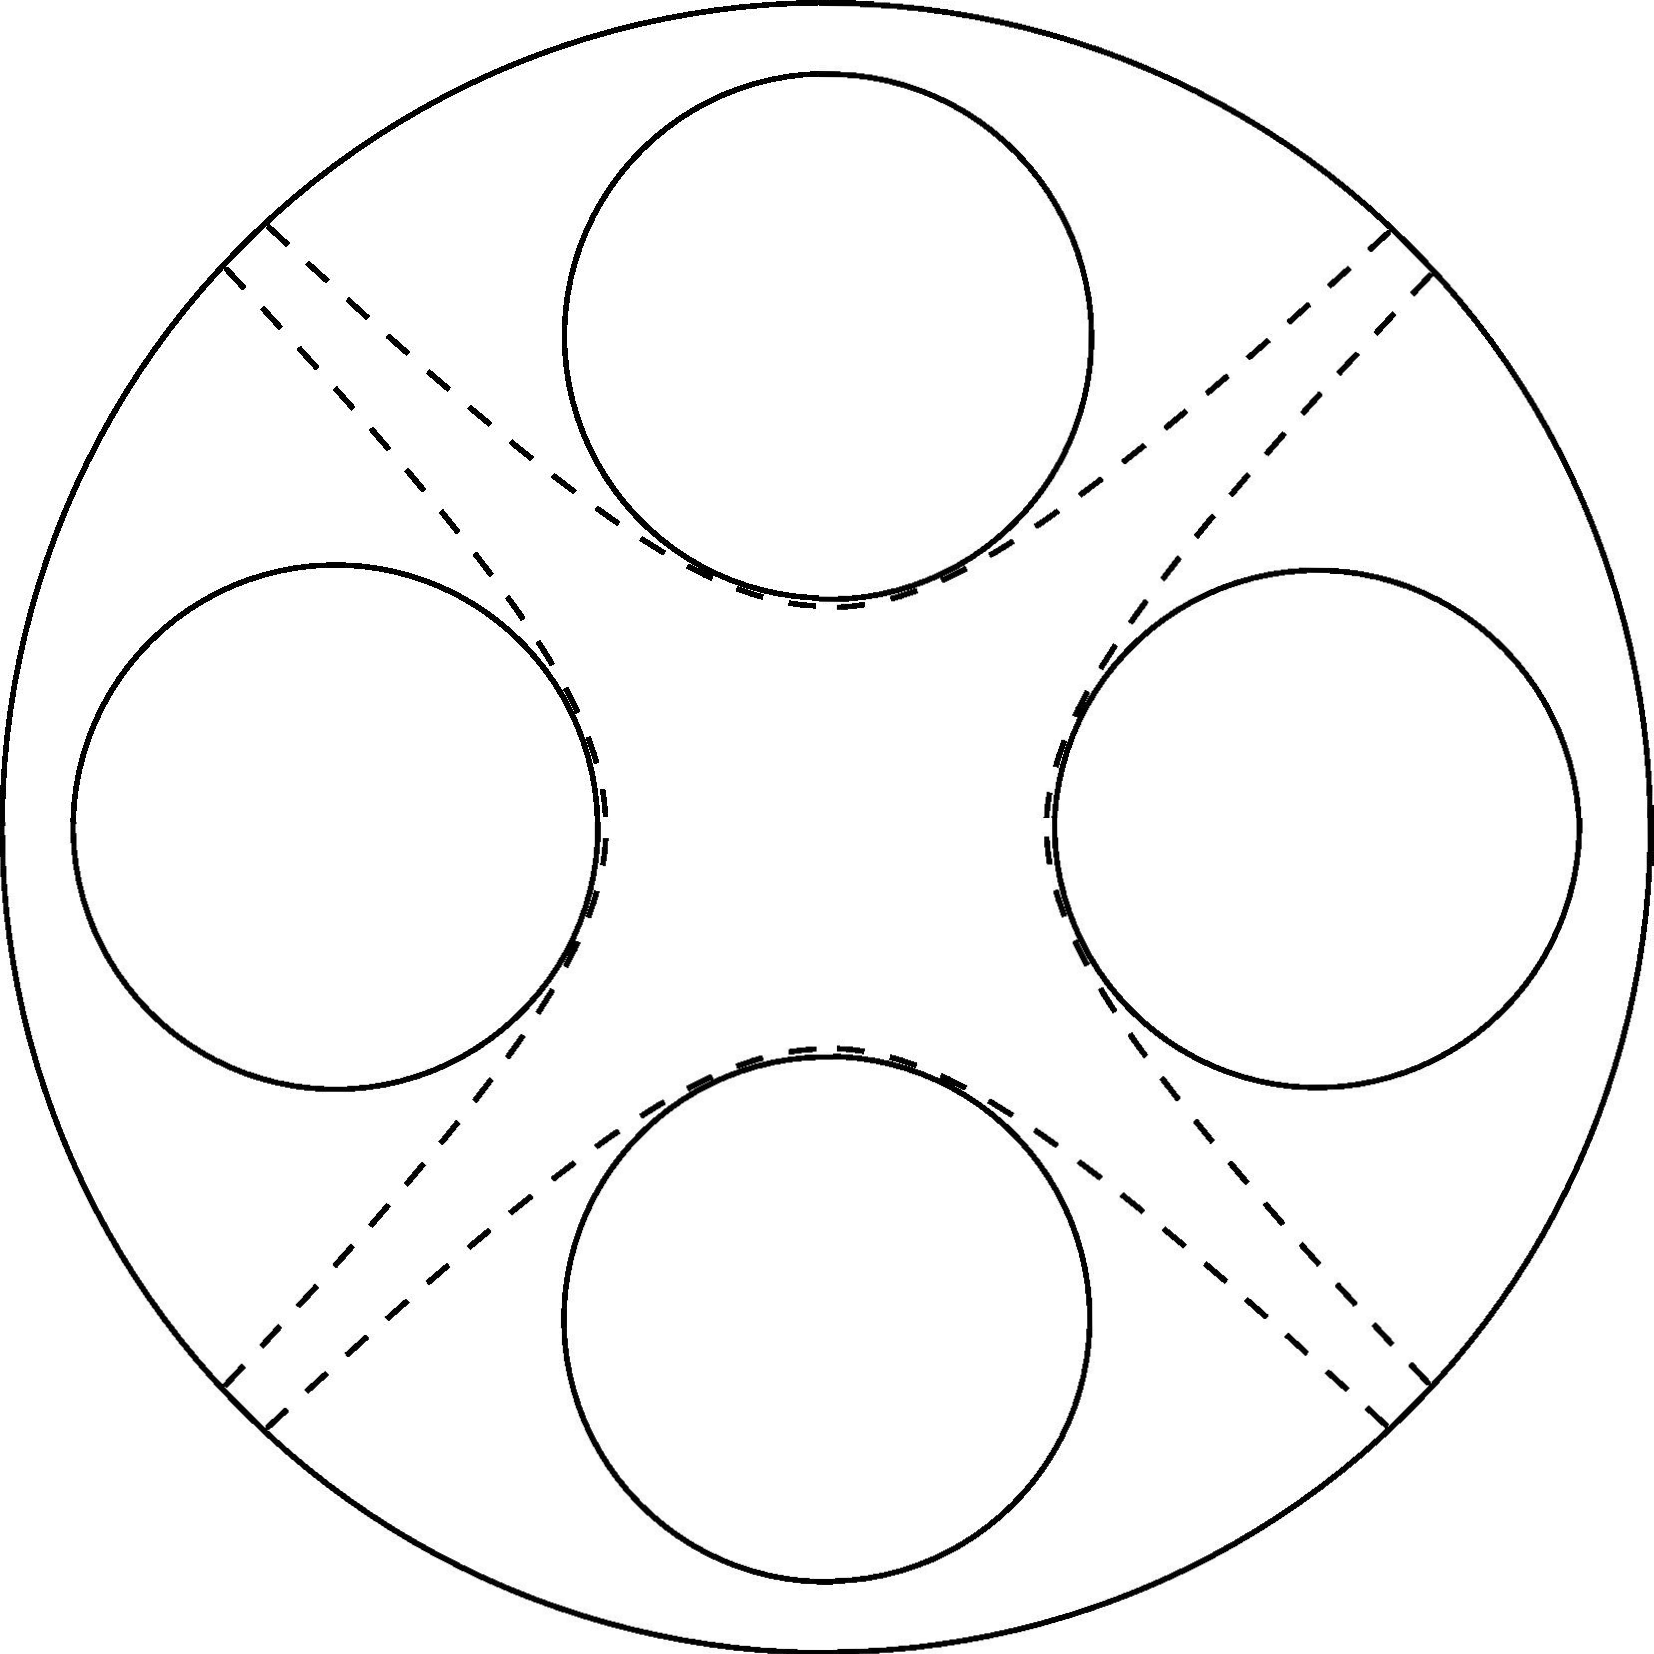
\includegraphics[width=\linewidth]{img/quadrupole_scheme.png}
	\caption{The scheme of quadrupole's cross-section. Adapted from \cite{FANGHANEL2017124}.}
	\label{fig:quadrupole scheme}
\end{subfigure}\hfill%
\begin{subfigure}{.47\textwidth}
	\centering
	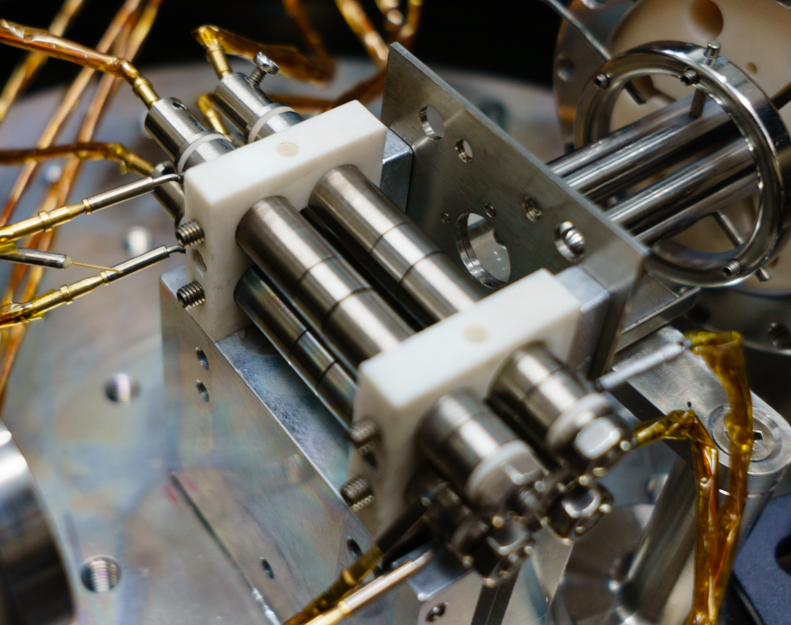
\includegraphics[width=\linewidth]{img/quadrupole.png}
	\caption{A photograph of linear quadrupole trap.}
	\label{fig:quadrupole picture}
\end{subfigure}
\caption{The quadrupole trap}
\label{fig:quadrupole}
\end{figure}
\todo{Do I need to cite somebody for \ref{fig:quadrupole picture}?}In the figure \ref{fig:quadrupole scheme}, we can see a comparison of a quadrupole trap's hyperbolical \textit{(dashed)} and linear \textit{(four circles)} electrode geometries. The quadrupole is already a very important geometry worth a special alias $\rightarrow$ the Paul trap, as will be pointed out shortly. We define a characteristic length of the multipole $\ell_0$, indicating the closest distance from the trap's center to an electrode. It is possible to obtain a potential of a multipole with infinitely long linear electrodes by applying boundary conditions \eqref{boundary condition n-pole} to a solution of Laplace equation with cylindrical symmetry \eqref{cylindrical symmetry potential}.
\begin{subequations}
\label{boundary condition n-pole}
\begin{align}
	\Phi(r,\varphi)\vert_{r=0}&=0, \\
	\Phi(r,\varphi)\vert_{r=\ell_0}&=\Phi_0 \cos(n\varphi),
\end{align}
\end{subequations}
where $\Phi_0 = V_0 + V_1 \cos(\Omega_1 t)$ is a potential applied on electrodes. Most of the coefficients in \eqref{cylindrical symmetry potential} get wiped out, and we end up with the potential of n-th order multipole $(n > 0)$ as:
\begin{equation}
	\label{potential n-pole}
	\Phi(r,\varphi) = \Phi_0 \hat{r}^n \cos(n\varphi),	
\end{equation}
where $\hat{r} = \nicefrac{r}{\ell_0}$. We get an electric intensity in polar coordinates as: 
\begin{equation}
	\vb{E}(r,\varphi) = \minus\nabla_{r\varphi} \Phi(r,\varphi),
\end{equation}
where $\nabla_{r\varphi} = \left[\dfrac{\partial}{\partial r}, \dfrac{1}{r} \dfrac{\partial}{\partial \varphi}\right]^\top$. Hence:
\begin{equation}
\label{need this for norm(E_0)}
\vb{E}(r,\varphi) = \dfrac{\Phi_0}{\ell_0} n \hat{r}^{n-1} 
\begin{bmatrix}
	\minus\cos(n\varphi) \\
	\sin(n\varphi)
\end{bmatrix},
\end{equation}
which in the Cartesian representation takes the form \cite{gerlich1992inhomogeneous}:
\begin{equation}
\begin{bmatrix}
	E_x \\
	E_y
\end{bmatrix}
 = \dfrac{\Phi_0}{\ell_0} n \hat{r}^{n-1} 
\begin{bmatrix}
	\minus\cos\big((n \minus 1)\varphi\big) \\
	\sin\big((n \minus 1)\varphi\big)
\end{bmatrix}.
\end{equation}
After substituting for $\Phi_0$ we get equation of motion in variable $\vb{\hat{r}} = [\nicefrac{x}{\ell_0},\nicefrac{y}{\ell_0}]^\top$:
\begin{equation}
	\label{eq of motion multipole}
	\dfrac{d^2\vb{\hat{r}}}{dt^2} + \dfrac{n Q}{M \ell_0^2}\left(V_0 + V_1\right)\cos(\Omega_1 t) \hat{r}^{n-1}
	\begin{bmatrix}
		\minus\cos\big((n \minus 1)\varphi\big) \\
		\sin\big((n \minus 1)\varphi\big)
	\end{bmatrix} = \vb{0}.
\end{equation}
We see that for the case $n = 2$ the equation of motion \eqref{eq of motion multipole} is linear. The same is clearly does not hold for $n > 2$. That is why the motion in a quadrupole trap is the easiest to describe, and we chose this geometry to study simultaneous electron-ion trapping in this thesis.

\subsubsubsection{Ideal quadrupole trap}
\label{sec:quadrupole trap}
We have already derived a equation of motion for single charged particle in a quadrupole trap $\rightarrow$ $n=2$ in \eqref{eq of motion multipole}. This equation gets further simplified by replacing linear electrodes with hyperbolical ones \ref{fig:quadrupole scheme}. With this change, the electric field gets scaled \cite{leefer2017investigation} by a factor $\nicefrac{1}{2}$, but foremost it loses the spatial dependence on the angle $\varphi$. In that case, the motion in the x and y directions stays independent, and we obtain an equation of motion in a variable $\vb{r} = [x,y]^\top$ for an idealized quadrupole trap:
\begin{equation}
	\label{eq of motion hyperbolic electrodes}
	M\vb{\ddot{r}} = \minus\dfrac{Q}{\ell_0^2} \big[V_0 + V_1 \cos(\Omega_1 t)\big] \vb{r}.
\end{equation}
It is possible to assemble a Paul trap for confinement in all directions. In that case, the same equation also describes motion in the z-direction, but with a rescaled right-hand side by the factor of $\minus 2$. We will take a closer look at the equation \eqref{eq of motion hyperbolic electrodes} in the section \ref{sec:mathieu equation}. While we are at it, we can take a step back and define the potential for the idealized quadrupole trap. Equation of motion in terms of such potential would be: $M\vb{\ddot{r}}(t) = \minus Q\nabla V(t,\vb{r})$, comparing with the \eqref{eq of motion hyperbolic electrodes} gives us desired potential:
\begin{equation}
	\label{ideal quadrupole potential}
	V(t,\vb{r}) = \left[V_0 + V_1 \cos(\Omega_1 t)\right] \dfrac{x^2+y^2 \minus 2z^2}{2\ell_0^2}.
\end{equation}
Another essential subject we are interested in is the effective potential for this geometry. For that, we need to evaluate for $E_0$ in the equation \eqref{effective potential}. The value of $\vb{E_0}$ can be easily derived from \eqref{need this for norm(E_0)}, where for our case $\Phi_0 = \nicefrac{V_1}{2}$, as:
\begin{equation}
	\label{norm(E_0)}
	E_0 = \dfrac{V_1}{\ell_0^2} \tilde{r},
\end{equation}
where we define $\tilde{r} \equiv \left[x, y, \minus 2 z\right]^\top$. Meaning the effective potential for ideal Paul trap is:
\begin{equation}
	\label{effective potential hyperbolic}
	V^*(\vb{r}) = \dfrac{Q^2 V_1^2}{4\ell_0^4 M \Omega_1^2} \tilde{r}^2 + Q\Phi_s = \dfrac{Q^2 V_1^2}{4\ell_0^4 M \Omega_1^2} \left(x^2 + y^2 + 4z^2\right) + Q\Phi_s.
\end{equation}

\subsubsection{Real geometry of our trap}
Since we want to implement laser cooling in our experiment, the Paul trap is not a viable option, as its apparatus would stand in the way of laser beams. For this reason, we will use surface electrodes where the particles levitate above the trap so that the ions will be accessible to us.
\begin{figure}[H]
\begin{subfigure}{.5\textwidth}
  \centering
  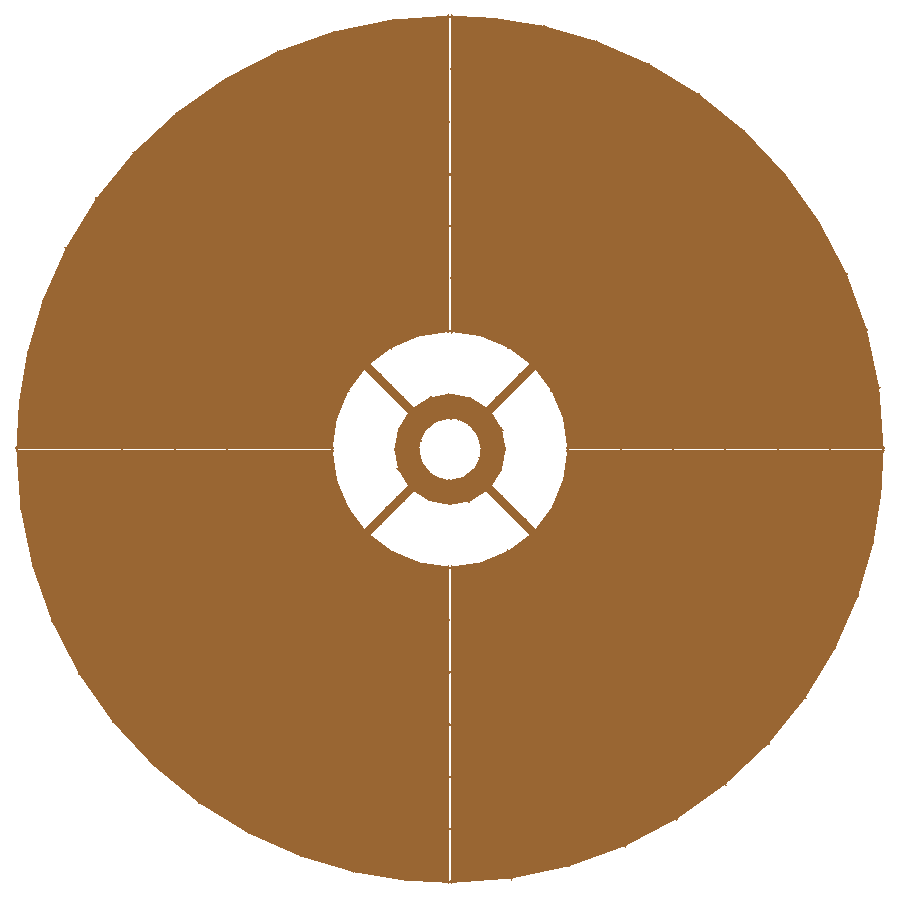
\includegraphics[width=\linewidth]{img/real_trap_geometry_1.pdf}
  \caption{Scheme of our planar trap.}
  \label{fig:Real trap geometry 1}
\end{subfigure}%
\begin{subfigure}{.5\textwidth}
  \centering
  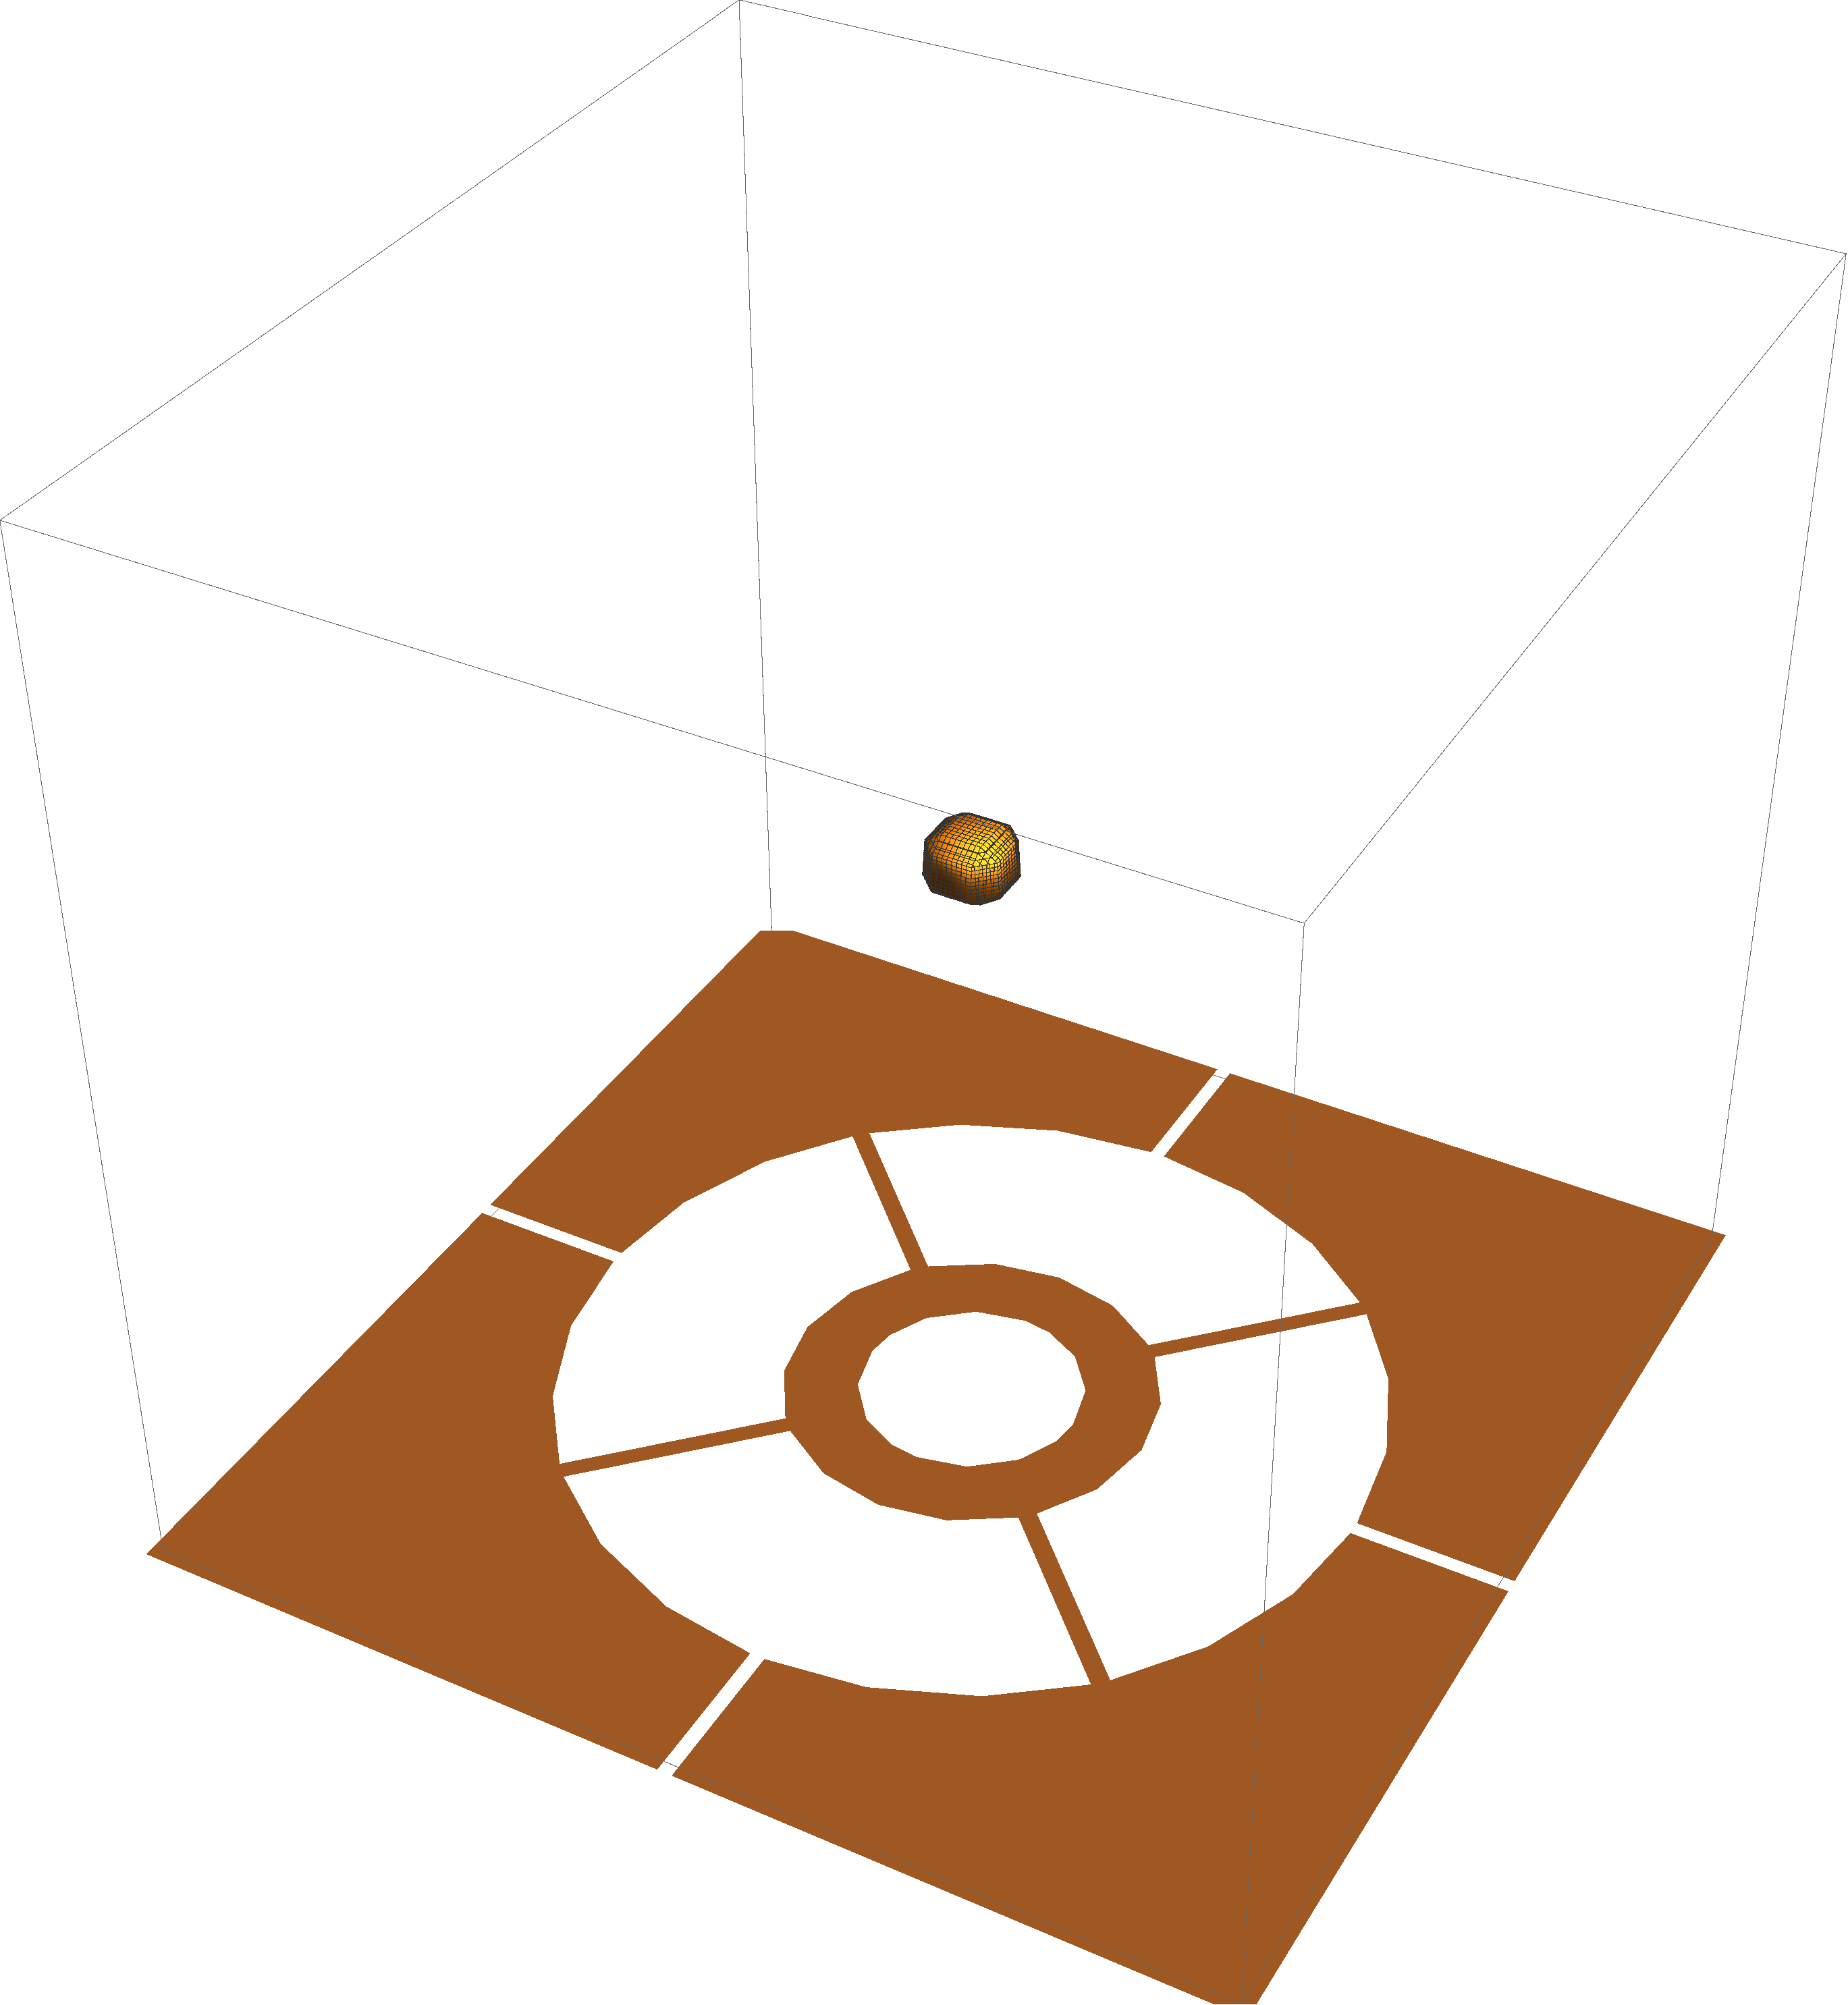
\includegraphics[width=\linewidth]{img/real_trap_geometry_2.pdf}  
  \caption{Our trap with calculated potential well above it (length in meters).}
  \label{fig:Real trap geometry 2}
\end{subfigure}
\caption{Planar trap geometry}
\label{fig:planar trap geometry}
\end{figure}
Nevertheless, we will conduct our research in this thesis by examining the situation with the geometry of the 3D quadrupole trap with hyperbolic electrodes.

\subsection{Spring constant}
\label{sec:spring constant}
If we focus on the dynamic component of an effective potential \eqref{effective potential hyperbolic}, we can see that it is formally equivalent to a potential of a harmonic oscillator\footnote{Meaning a potential in the form: $V(\xi) = \dfrac{\kappa}{2} \xi^2$}. This encourages us to define a spring constant: 
\begin{equation}
	\label{spring constant}
	\kappa \equiv \dfrac{Q^2 V_1^2}{2\ell_0^4 M \Omega_1^2},
\end{equation}
characterizing the strength of trapping potential. The spring constant is closely related to a frequency of oscillation in a harmonic potential. Such frequency is called secular, denoted: 
\begin{equation}
	\label{secular frequency}
	\omega \approx \sqrt{\nicefrac{\kappa}{M}} = \nicefrac{Q V_1}{\sqrt{2}\ell_0^2 M \Omega_1}.
\end{equation}
The good news is that the spring constant does not depend on the charge sign, making it possible to trap electrons as well as ions. The bad news is that the spring constant depends on the charge-to-mass ratio $\nicefrac{Q}{M}$, making it practically very difficult to trap electrons and ions simultaneously. For our case of trapping $Ca^+$ ions together with electrons, we get $\nicefrac{\kappa_{electron}}{\kappa_{ion}} = \nicefrac{M_{ion}}{M_{electron}} \approx 73000$ while we would like to achieve $\nicefrac{\kappa_{electron}}{\kappa_{ion}} \sim 10$ so that electron trajectories would ideally stay inside the ion crystal but at similar scales. It seems that we have hit upon a huge snag with our approach. Fortunately, we do not have to abandon the discussed concept for trapping. We can instead improve on it by adding a second frequency. Such change allows us to treat both species' stability individually and makes it possible to manage the desired ratio of spring constants. Two frequency Paul trap will be further discussed in section \ref{sec:two frequency trap}.

\subsection{Mathieu equation}
\label{sec:mathieu equation}
Let us reexamine our original equation of motion \eqref{equation of motion} for the case of a quadrupole trap with ideal hyperbolical electrodes. After time transformation $\tau = \nicefrac{\Omega_1 t}{2}$, the equation \eqref{eq of motion hyperbolic electrodes} molds into:
\begin{equation}
	\label{mathieu equation}
	\vb{\ddot{r}}(\tau) = \left[a \minus 2 q_1 \cos(2 \tau)\right] \vb{r},
\end{equation}
where:
\begin{subequations}
\begin{align}
	a &= \dfrac{4 Q V_0}{M \ell_0^2 \Omega_1^2}, \\
	q_1 &= \minus\dfrac{2 Q V_1}{M \ell_0^2 \Omega_1^2}.
\end{align}
\end{subequations}
The equation \eqref{mathieu equation} bears a name after E.L. Mathieu, who was the first to extensively study this ordinary differential equation(ODE) in the context of vibrating membranes. It has an analytical solution \cite{5416839} in terms of special functions called Mathieu functions, denoted $ce_n$ and $se_n$, sometimes referred to as cosine-elliptic and sine-elliptic. The secular frequency is given by \cite{gerlich1992inhomogeneous} the Dehmelt approximation:
\begin{equation}
	\omega \approx \frac{\Omega_1}{2} \sqrt{a + \frac{q_1^2}{2}}.
\end{equation}
If we do not apply any static field \textit{(as in is the case for our configuration)} the secular frequency is:
\begin{equation}
	\omega \approx \frac{\Omega_1}{2} \sqrt{\dfrac{q_1^2}{2}} = \dfrac{Q V_1}{\sqrt{2}\ell_0^2 M \Omega_1},
\end{equation}
which is in accordance with the result we attained with the spring constant in the harmonic pseudopotential.

\subsection{Stability} 
The stability of a linear system such as \eqref{mathieu equation} can be examined with the help of a robust theory for linear ODEs with periodic coefficients, which we do in section \ref{sec:floquet theory}. Nevertheless, we eventually want to study the trapping of multiple charged particles, and their mutual interaction razes the linearity of our equations. There is no single outright mathematical way to define the stability of a non-linear, non-autonomous system. Mathematical approaches might demand the boundedness of the solution in the phase space. Then we would talk about Lagrange stability \cite{bhatia2002stability}. Another approach would be to seek stable points and study what happens to the solutions starting in their proximity. This approach is referred to as Lyapunov stability \cite{lyapunov1992general}. We will use a simple but practical criterion for identifying stable solutions. A stable particle cannot vacate the internal dimension of the trap, meaning:
\begin{equation}
	\max\limits_{x \in \mathcal{L}}(r) \leq r_m < \ell_0,
\end{equation}
where $\mathcal{L}$ is the whole trajectory of the particle and $r_m$ is maximal allowed distance from the center of a trap. The drawback of this definition is that we must keep the simulation going long enough to account for the slowly diverging particles, and we are yet to determine the value of $r_m$. However, we can also characterize the mode for stable confinement in a more general manner \cite{gerlich1992inhomogeneous}. First, we limit ourselves to work within the condition for adiabaticity to ensure that the dynamic field does not continually augment the particle's energy. Then we can exploit the equation \eqref{adiabatic constant} in the following way. A stable particle must have no secular momentum $\vb{\dot{R}_0} = \vb{0}$ at the point $r_m$ to avoid collision with the electrode. The effective potential near the electrode must be greater than the adiabatic constant $E_m$. Otherwise, the potential will not be powerful enough to prevent rapid oscillatory motion from ejecting the particle out of the trap. Giving us the applicable inequality for stable confinement:
\begin{equation}
	\label{stability condition inequality}
	\dfrac{Q^2 E_0^2(r_m)}{4 M \Omega^2} + Q\Phi_s > E_m.
\end{equation}
We still need to find the right value for $r_m$. It has been established \cite{gerlich1992inhomogeneous} that $r_m = 0.8 \ \ell_0$ accomplishes adiabaticity for most cases, which we will also use as a stability condition in our simulations:
\begin{equation}
	\label{stability condition in simulation}
	\max\limits_{x \in \mathcal{L}}(r) \leq 0.8 \ \ell_0.
\end{equation}

\section{Laser cooling}
We demonstrate the principle of laser cooling on a calcium ion. The $Ca^+$ ion has an energy gap between the ground $(S_{\nicefrac{1}{2}})$ and one of its excited $(P_{\nicefrac{1}{2}})$ states with the value corresponding to the wavelength of $\SI{397}{\nano\meter}$ \cite{urabe1993laser}. By tuning the wavelength of our laser slightly below this transition energy, we can exploit the Doppler effect so that only ions moving towards the laser can experience radiation with the right frequency to excite them. After a brief time, the atom will deexcite, emitting a photon in a random direction. The only way the ion would still have the same momentum as before the absorption is if the photon was emitted exactly in the same direction as it was absorbed (as if the photon did not interact with the atom at all). But since the photon emission is isotropic, the ion will effectively slow down. This type of laser cooling is also known as \emph{Doppler cooling}. Detailed explanation can be found in \cite{alma990008711500106986}.   

\section{Design of the experiment}

As we have already stated, we chose a planar trap geometry, offering easy access to ions for laser cooling. Creating such a trap is a challenge in itself, and we have other colleagues in our team devoted to completing this task. Here we offer a quick overview of its development. Our circuit material is made of borosilicate glass for practical reasons. On it, we need to deposit a layer of copper by electroplating, forming the electrodes of our trap. Here arises the first problem, as the copper suffers from poor adhesion on the smooth surface of the glass. There are many ways to overcome this issue. We chose a straightforward one by roughening the glass mechanically with lasers.
\begin{figure}[H]
\begin{subfigure}{.45\textwidth}
	\centering
	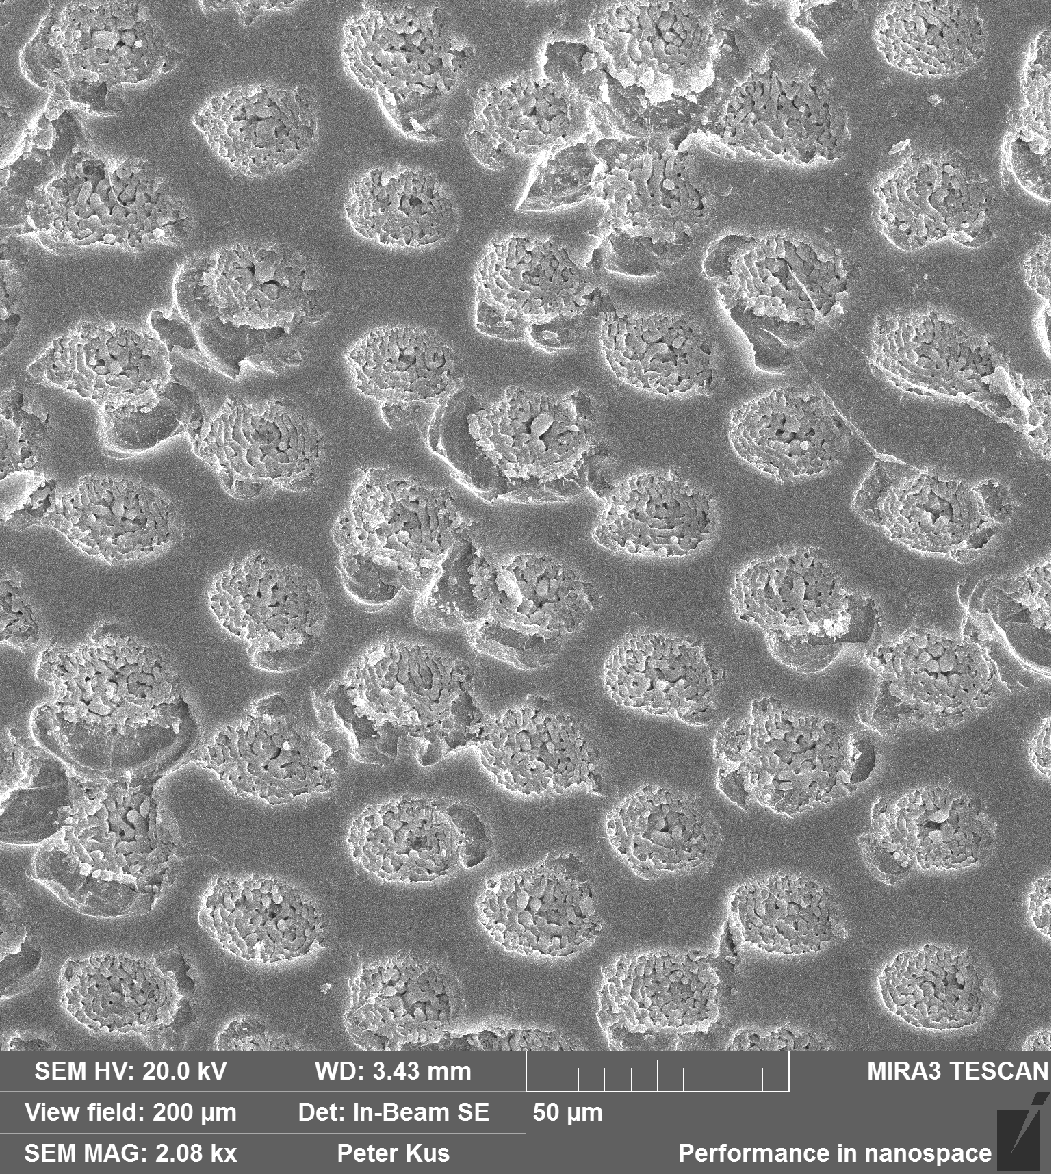
\includegraphics[width=\linewidth]{img/200um_glass.pdf}
	\caption{The surface of the glass after the laser roughening.}
	\label{fig:glass}
\end{subfigure}\hfill%
\begin{subfigure}{.465\textwidth}
	\centering
	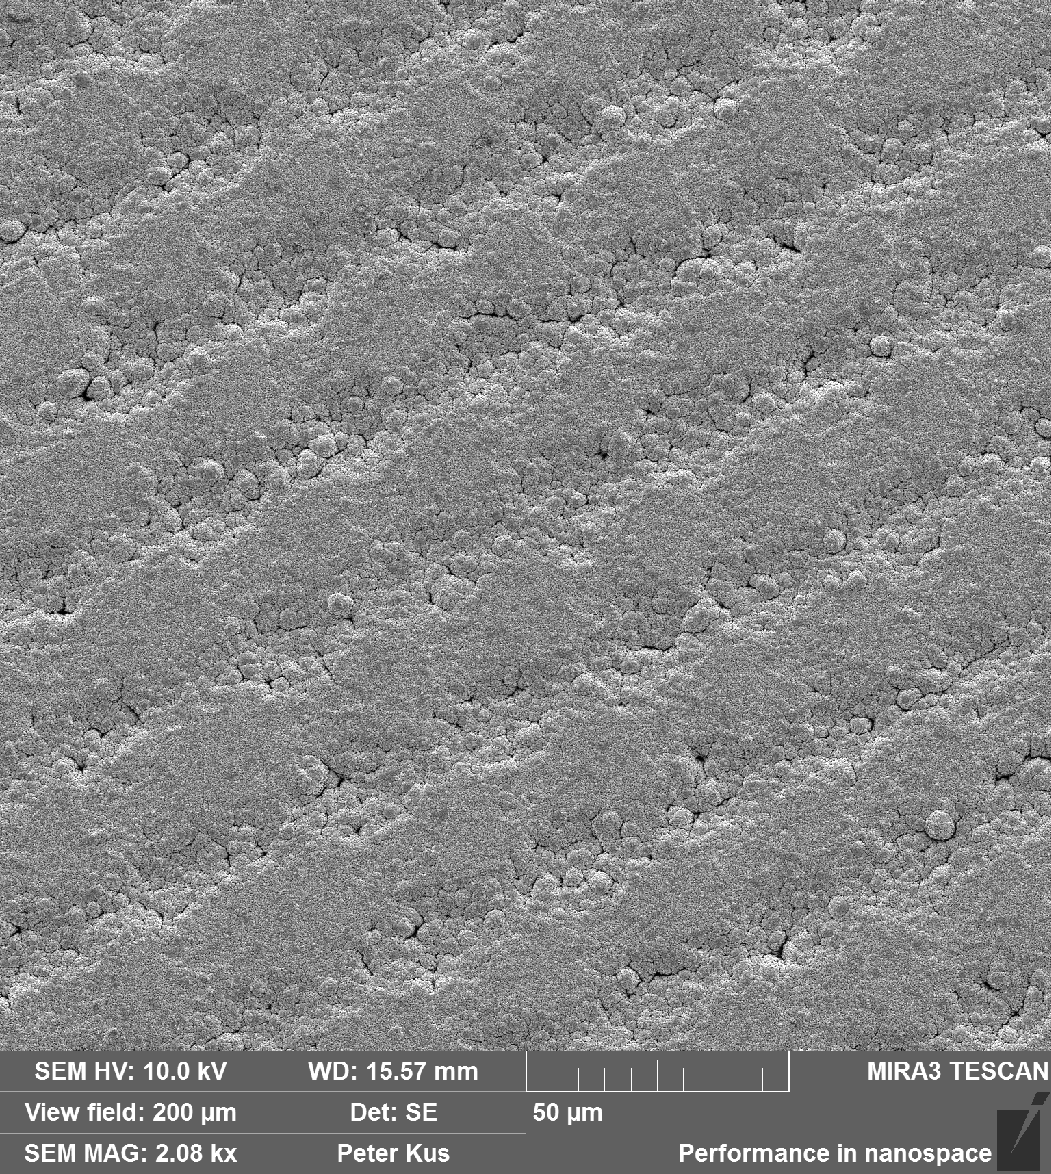
\includegraphics[width=\linewidth]{img/200um_copper.pdf}
	\caption{A copper layer on the glass.\\}
	\label{fig:quadrupole picture}
\end{subfigure}
\caption{Pictures of our electrode manufacturing taken by an electron microscope.}
\label{fig:trap manufacturing}
\end{figure}
We also use lasers to cut ways for the connection of each electrode to the power source. Next, we need a source of calcium ions. We manage that by evaporation from a calcium rod under a high voltage. Evaporated atoms will be excited by a $\SI{397}{\nano\meter}$, laser creating a desired ion $Ca^+$ and an electron. For cooling, we use two lasers. The first is the same as we use for photo-ionization. The second with a wavelength of $\SI{866}{\nano\meter}$ is necessary for cooling to lower temperatures, exploiting another transition of calcium ion between the state $(P_{\nicefrac{1}{2}})$ and the meta-stable state $(D_{\nicefrac{3}{2}})$. Of course, such a complex experiment is met with dozens of other technical issues, but those are outside the scope of this thesis.